\chapter{Метод CLIP-ReID}
\label{ch:clipreid}

Как упоминалось ранее, для эффективного применения технологий Re-Id в системе поиска, необходимо использовать методы, обрабатывающие на ряду с визуальной информацией некоторую дополнительную. В данном разделе рассмотрим принцип работы state-of-the-art метода решения задачи \reid\ CLIP-ReID \cite{li2023clip}. Он показывает наилучшее качество на одном из бенчмарков задачи ReId $-$ MSMT17 \cite{wei2018person}. Он опирается на мультимодальную модель CLIP \cite{radford2021learning}, позволяющую строить эмбеддинги изображений и текстовых описаний к ним в одном и том же метрическом пространстве. Также здесь применяется техника \textit{prompt tuning}, используемая в методе обучения классификации CoOp \cite{zhou2022learning}, для построения более состоятельных представлений с помощью обучения как визуальной, так и текстовой частей модели CLIP. Схема работы этих методов представлена на \hyperref[fig:clipreid]{Рисунке \ref*{fig:clipreid}}.

\begin{figure}[ht]
	\centering
	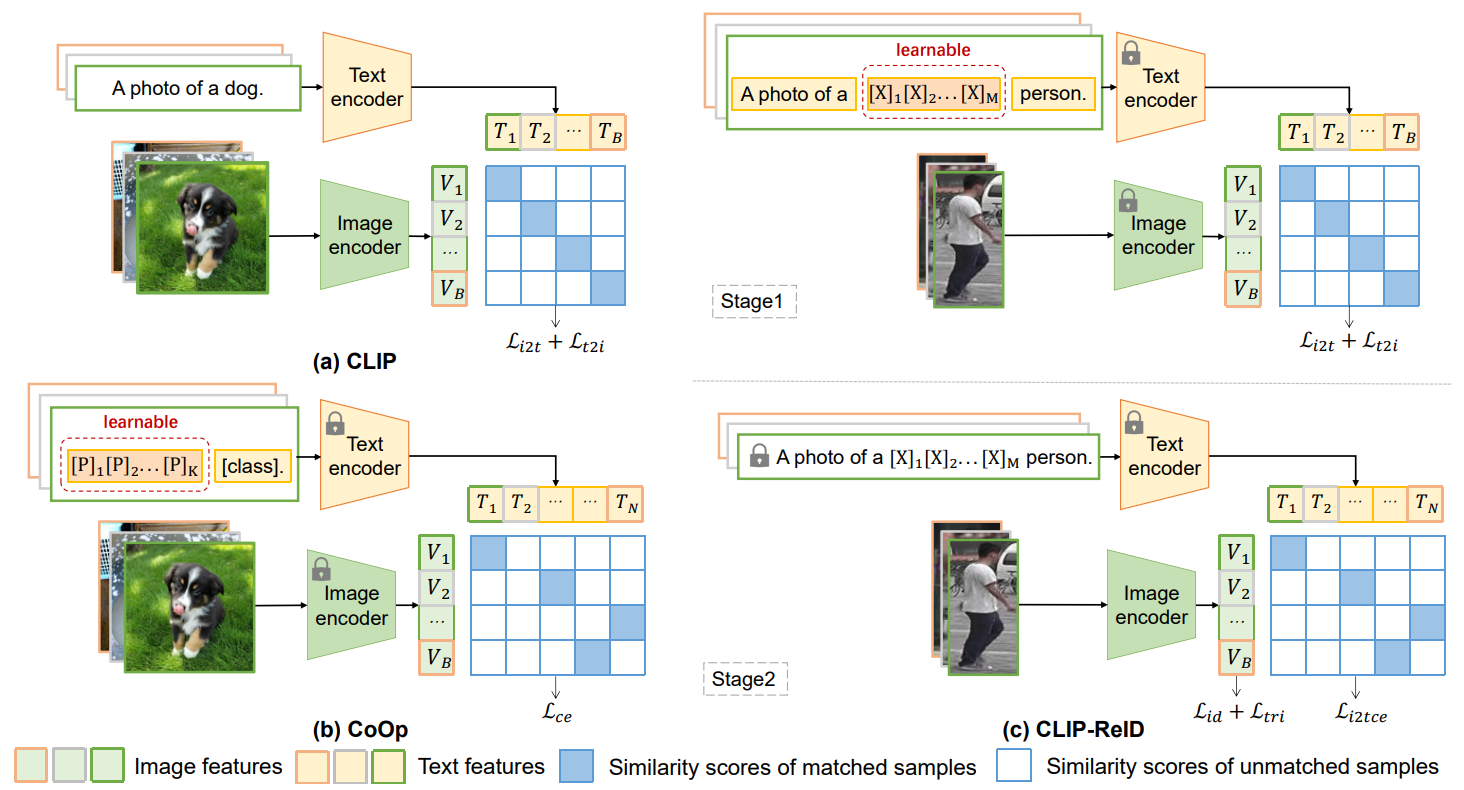
\includegraphics[width=0.9\textwidth]{images/clipreid/scheme.png}
	\caption{Схема работы методов CLIP и CLIP-ReID \cite{radford2021learning}, \cite{li2023clip}}
	\label{fig:clipreid}
\end{figure}


\section{CLIP}

Суть подхода CLIP состоит в построении мультимодальной модели, содержащей энкодер изображений $\mathcal I(\cdot)$ и текстовый энкодер $\mathcal T(\cdot )$. В качестве архитектуры визуального энкодера используется два варианта: ResNet и ViT. В качестве текстового энкодера используется трансформер. Для построения эмбеддинга изображения используется выход визуального энкодера, а для в качестве текстового эмбеддинга выдается представление позиции конца последовательности после преобразования текста трансформером. Затем эти два эмбеддинга проецируются в пространства одинаковой размерности для получения совместных метрических представлений.

Далее на полученные эмбеддинги накладываеются функции потерь, направленные на установление соответствия эмбеддингов текста и картинки, соответствующих одному и тому же объекту. Для объекта батча с индексом $i \in \overline{1, B}$ обозначим текстовое и визуальное представления соответственно $T_i$ и $V_i$. Далее для каждой пары объектов $i$, $j$ считается похожесть, исходя из скалярного произведения:

\begin{equation}
	s (V_i, T_j) = V_i \cdot T_j.
\end{equation}

Лос-функция $\mathcal L_{i2t}$ представляет собой кросс-энтропию, накладываемую в соответствии с классификацией каджого визуального эмбеддинга по похожести с текстовыми эмбеддингами:

\begin{equation}
	\mathcal L_{i2t}(i) = - \log \frac{\exp \left( s(V_i, T_i) \right)}{\sum_{j = 1}^B \exp \left( s(V_i, T_j) \right)}.
\end{equation}

Аналогично определяется функция потерь $\mathcal L_{t2i}$, отвечающая за соответствие текстовых эмбеддингов визуальным:

\begin{equation}
	\mathcal L_{t2i}(i) = - \log \frac{\exp \left( s(V_i, T_i) \right)}{\sum_{j = 1}^B \exp \left( s(V_j, T_i) \right)}.
\end{equation}

Далее они объединяются в итоговую функцию потерь с помощью суммирования:

\begin{eqnarray}
	\mathcal L = \mathcal L_{i2t} + \mathcal L_{t2i}.
\end{eqnarray}

Данный подход позволяет получить модель, способную решать сложные задачи соответствия между текстовыми описаниями и визуальными характеристиками объектов. 

Один из вариантов его развития $-$ метод CoOp, применяющий обучение промптов вместо текстовых описаний при сохранении фиксированными параметров текстового и визуального энкодеров. Данный подход позволяет настравивать CLIP на различные прикладные задачи, связанные с классификацией. Однако для задачи ре-идентификации этот метод не дает прямых преимуществ по сравнению с исходной моделью CLIP, поскольку в отсутствие конкретных текстовых описаний, а также незафиксированном множестве классов, имеется необходимость настройки визуальных эмбеддингов, а не промптов.


\section{CLIP-ReID}

В свою очередь, метод CLIP-ReID адресуется к задаче ре-идентификации. Для этого вводится две стадии настройки предобученной модели CLIP. Авторы показывают, что каждая из этих стадий вносит значимый вклад в прирост качества решения задачи.

\subsection{Первая стадия обучения}

На этом этапе параметры текстового и визуального энкодеров фиксируются. Обучаемыми остается отдельный модуль, называемый \textit{prompt learner} $\mathcal P(\cdot)$. Он формирует входные данные для энкодера $\mathcal T(\cdot)$. Так, для каждого человека, представленного в датасете, формируется описание в формате "A photo of a $[X]_1[X]_2\dots[X]_m$ person". Здесь $[X]_i$ представляет собой обучаемые эмбеддинг токена. Так, при подаче в модель текст разбивается на токены специальным токенизатором, предоставляемым CLIP; для каждого токена строится эмбеддинг. Для токенов $[X]_i$ реальных текстовых токенов нет, именно их представление в виде эмбеддинга является обучаемым параметром модели. 

Каждому человеку соответствует своя обучаемая последовательность эмбеддингов. При этом в батче могут содержаться изображения, соответствующие одному и тому же человеку, поэтому на данном этапе функция потерь модифицируется для учета этого факта:

\begin{equation}\label{eq:Lt2i}
	\mathcal L_{t2i}(y_i) = \frac{-1}{|P(y_i)|} \sum \limits_{p \in P(y_i)} \log \frac{\exp \left( s(V_p, T_{y_i}) \right)}{\sum_{j = 1}^B \exp \left( s(V_j, T_{y_i}) \right)}.
\end{equation}

Итоговая функция потерь также представляет собой сумму текстовой и визуальной кросс-энтропий:

\begin{eqnarray}
	\mathcal L_{stage1} = \mathcal L_{i2t} + \mathcal L_{t2i}.
\end{eqnarray}

Здесь $P(y_i)$ $-$ множество объектов, соответствующих тому же человеку $y_i$. Таким образом с помощью обратного распространения ошибки параметры эмбеддингов промптов оптимизируются для формирования информативных представлений.

\subsection{Вторая стадия обучения}

На втором этапе обучения фиксируются параметры $\mathcal P(\cdot)$ и настраиваются параметры визуального энкодера $\mathcal I(\cdot)$. Здесь совмещаются основные техники решения задачи \reid. Одно из слагаемых представляет собой триплет-лосс:

\begin{equation}\label{eq:Ltri}
	\mathcal L_{tri} = \max \left( d_p - d_n + \rho, 0 \right).
\end{equation}

Второе из слагаемых представляет собой softmax-loss с применением техники сглаживания лейблов, или \textit{label-smoothing},  то есть замены целевого единичного вектора на вектор с малыми, но ненулевыми, значениями на позициях нулей и разности единицы с их суммой на позиции единицы:

\begin{equation}\label{eq:Lid}
	\mathcal L_{id} = \sum \limits_{k = 1}^N q_k \log(p_k),
\end{equation}

где $N$ - количество человек, представленных в датасете, сглаженный индикатор $q_k = (1 - \varepsilon) \delta_{k, y} + \varepsilon N$. Наконец, третье слагаемое отвечает за построение более состоятельных эмбеддингов, соответствующих текстовым промптам. Здесь также используется label smoothing:

\begin{equation}\label{eq:Li2tce}
	\mathcal L_{i2tce}(i) = \sum \limits_{k = 1}^N -q_k \log \frac{\exp \left( s(V_i, T_{y_k}) \right)}{\sum_{y_j = 1}^N \exp \left( s(V_i, T_{y_j}) \right)}.
\end{equation}

Итоговая функция потерь в таком случае:

\begin{equation}
	\mathcal L = \mathcal L_{tri} + \mathcal L_{id} + \mathcal L_{i2tce}(i).
\end{equation}

Таким образом, на первой стадии происходит установка соответствий между информацией, заложенной в предобученную модель CLIP, в виде текстовых промптов. На второй же стадии они применяются в качестве регуляризатора для настройки визуальной модели, позволяя использовать все преимущества мультимодальной модели CLIP.






